\documentclass[11pt,letterpaper]{article}
\usepackage[left=1in,right=1in,top=0.9in,bottom=0.9in]{geometry}
\usepackage[T1]{fontenc}
\usepackage[utf8]{inputenc}
\usepackage{lmodern}
\usepackage{microtype,amsmath,booktabs,tabularx,longtable,array,graphicx,placeins,float}
\usepackage{titlesec,needspace}
\usepackage[font=small,labelfont=bf,labelsep=period,justification=justified,singlelinecheck=false]{caption}
\usepackage[numbers,sort&compress]{natbib}
\usepackage{xurl}
\usepackage[hidelinks]{hyperref}
\graphicspath{{figures/}}
\linespread{1.04}
\setcounter{secnumdepth}{3}
\setlength{\parindent}{0pt}
\setlength{\parskip}{0.3em plus 0.05em minus 0.02em}
\setlength{\emergencystretch}{2em}
\titleformat{\section}{\large\bfseries}{\thesection}{0.7em}{}
\titleformat{\subsection}{\normalsize\bfseries}{\thesubsection}{0.7em}{}
\titlespacing*{\section}{0pt}{1.3\baselineskip}{0.55\baselineskip}
\titlespacing*{\subsection}{0pt}{0.9\baselineskip}{0.35\baselineskip}
\captionsetup{skip=7pt}
\captionsetup[table]{position=top,skip=6pt}
\setlength{\abovedisplayskip}{9pt plus 2pt minus 2pt}
\setlength{\belowdisplayskip}{9pt plus 2pt minus 2pt}
\clubpenalty=10000
\widowpenalty=10000
\displaywidowpenalty=10000
\raggedbottom
\setlength{\textfloatsep}{12pt plus 2pt minus 2pt}
\setlength{\intextsep}{12pt plus 2pt minus 2pt}
\renewcommand{\topfraction}{.9}
\renewcommand{\bottomfraction}{.8}
\renewcommand{\textfraction}{.1}
\renewcommand{\floatpagefraction}{.8}
\hypersetup{pdftitle={Learning to Allocate Risk in Options Markets},
 pdfauthor={Adam Kreitzman and Soo Xin Yang}}
\begin{document}
\begin{center}
\makebox[\textwidth][c]{{\fontsize{19}{23}\selectfont\bfseries Learning to Allocate Risk in Options Markets}}
\vspace{0.6em}

{\fontsize{11}{14}\selectfont Contextual Position Sizing and Q-Learning for Capital Allocation}\par
\vspace{1em}
Adam Kreitzman and Soo Xin Yang\par
{\small 20 October 2026}
\end{center}
\begin{center}
\begin{minipage}{0.88\textwidth}
\small
\begin{center}\bfseries Abstract\end{center}
\setcounter{secnumdepth}{3}
\setlength{\parindent}{0pt}\noindent
We study two exposure decisions in equity options: contextual position sizing within strategies and capital allocation between strategies with fitted Q-learning. Contract-level simulations separately construct portfolios of approximately 30-day, 25-delta put pairs and short ATM straddles selected by persistent realized-minus-implied volatility. A separate allocator reallocates capital between fractional claims on the funded strategy return indices, rather than a shared contract inventory. During January 2022--August 2025, learned entry sizing raises annualized excess Sharpe from 1.055 to 1.263 for put pairs and from 0.990 to 1.041 for straddles, relative to full sizing. At the illustrative risk preference \(\lambda=0.20\), combining both learners raises Sharpe from 1.088 to 1.726 in a four-way comparison. The original validation-selected Q policy instead achieves later Sharpe 0.282, so the illustrative gain does not establish successful validation-based policy selection. With learned-size entries, Q also exceeds rolling mean--variance allocation: 1.726 versus 1.519. Interpretation connects entry decisions to completed profitability and volatility, and strategy allocation to the changing reward for straddle risk. Statistical uncertainty and assumed execution quality qualify these historical results.
\end{minipage}
\end{center}
% Introduction and related work are inline; the remaining source is organized by strategy.
\section{Introduction}\label{sec:1}
Finding a useful trading signal leaves an investor with a second problem: how much capital should it receive as opportunities and risks change? In options markets, a strategy with favorable risk-adjusted returns can deploy little capital, while a strategy that earns more dollars can expose the account to much larger movements. A ranking of average returns or Sharpe ratios alone does not determine when either strategy deserves funding. We study whether information available at the time of a decision can improve that allocation.

We make the question concrete with two equity-options strategies. The first buys relatively cheap puts and sells relatively expensive puts on related names, using approximately 30-day, 25-delta contracts. It matches vega at entry and adjusts stock delta hedges daily, while retaining differences in realized paths, jumps and company-specific events. The second sells approximately 30-day ATM straddles on names whose completed historical outcomes show persistently low realized volatility relative to entry implied volatility. It also hedges delta daily, but retains net short-gamma and short-vega exposure. These are different sources of option risk: relative pricing across names and premium income against future movement.

Our central learning question is how to allocate capital between the resulting portfolios. A fitted Q-learning policy chooses weekly capital targets using current opportunity measures, completed strategy performance, risk conditions and previous holdings. Entry sizing supplies a supporting decision within each strategy: contextual sizing policies choose 50\%, 75\% or 100\% of a proposed trade's full size. These sizing policies are fitted in batches to completed outcomes and optimize aggregate profit paths; they do not implement an online exploration-and-reward update. The economic rules determine proposals, directions and contracts; the entry policies alter commitments and subsequent admission capacity, while the allocation policy changes the capital assigned to each funded strategy index.

\begin{figure}[!htbp]\centering
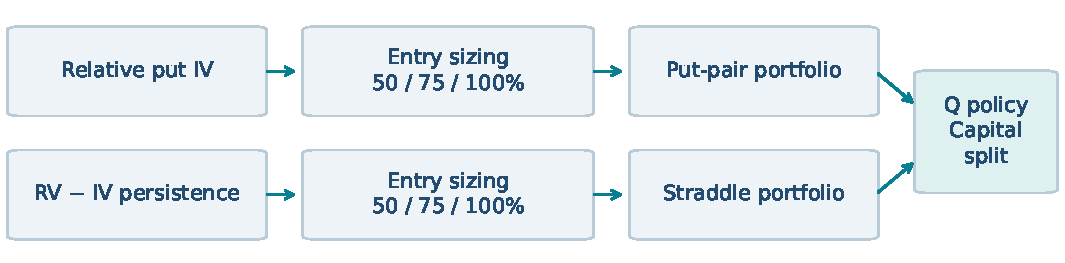
\includegraphics[width=\linewidth]{learning_pipeline.pdf}
\caption{Two exposure decisions. Entry policies size proposals within each signal; a separately fitted Q policy chooses the capital split between funded strategy indices.}\label{fig:learning-pipeline}
\end{figure}

We evaluate these decisions through actual-contract simulations with option marks, daily stock hedges, financing and explicit trading charges. A four-way comparison evaluates full-size entries with fixed 50/50 allocation, learned-size entries with fixed 50/50 allocation, full-size entries with Q allocation, and learned-size entries with Q allocation. All four receive the same signal proposals, and Q is independently refitted for each entry-policy family. During January 2022--August 2025, annualized excess Sharpe rises from 1.088 with full-size entries and fixed 50/50 allocation to 1.726 with both learners at the illustrative risk preference \(\lambda=0.20\). The original validation-selected policy has later Sharpe 0.282; the headline comparison illustrates allocation behavior rather than successful transfer of the validation selection. With learned-size entries, Q also exceeds rolling mean--variance allocation, 1.726 versus 1.519. Timing and one-period controls investigate whether the allocation result reflects average exposure, conditional information or continuation value; they indicate a larger role for conditional allocation and a smaller incremental sequential benefit. These comparisons describe a profit--risk tradeoff, with no single policy dominating every entry size, risk preference or performance measure.

Both 2018--2021 validation and January 2022--August 2025 evaluation remain visible throughout. Individual fits use strictly completed past outcomes; whether and how later-period results informed development remains under verification in Section~\ref{app:research-chronology}. The evaluation is treated as researched historical evidence rather than a confirmed independently frozen test of the complete research process. Statistical uncertainty and assumed execution quality qualify the performance gains. The outer allocator also trades fractional claims on separately funded strategy indices; it does not rebuild a shared whole-contract inventory. Our contribution is a controlled examination of adaptive exposure allocation under these assumptions, motivating integrated implementation and prospective evaluation.
\section{Related Work}\label{sec:2}
Ning and Lee \cite{ning2024} combine equity-spread construction with tabular Q-learning for entry and exit. They select hedge coefficients by minimizing empirical mean-reversion time and train the trading policy on simulated Ornstein--Uhlenbeck spreads. Evaluation on ten US equity pairs, formed in 2022 and traded in 2023, yields higher reported daily Sharpe ratios than their distance-method and Ornstein--Uhlenbeck benchmarks. Their analysis focuses on entry and exit within a constructed equity spread; it does not examine capital allocation across distinct options strategies. We study that allocation decision using relative-value put pairs and short ATM straddles, with controlled comparisons that separate learned entry sizing from learned strategy allocation.

Bell et al. \cite{alphaglass2026} develop AlphaGlass, an interpretable framework that maps stock characteristics into additive signals with sparse interactions and converts those signals into long--short portfolio weights through a differentiable rank-and-mask layer. The model is trained against portfolio objectives such as Sharpe or mean--variance utility, linking the learned signal directly to the investor's objective. Its additive structure makes portfolio weights traceable to individual characteristics and interactions. This combination of objective-based learning and interpretable decisions connects to our completed-path Sharpe optimization and policy diagnostics. The decision structures differ: AlphaGlass learns characteristic-based equity portfolio weights, whereas our fixed options signals generate candidate trades, contextual policies size those trades, and fitted Q-learning allocates capital across the resulting strategy portfolios.

Halperin \cite{halperin2017qlbs} introduces QLBS, a discrete-time framework for option pricing and hedging based on a risk-adjusted Markov decision process. Q-learning jointly determines option values and hedge decisions by optimizing the risk-adjusted performance of a replicating portfolio, with a data-driven formulation that can learn from observed paths. QLBS provides a precedent for Q-learning in an options setting, but addresses a different control problem. Our option valuation and daily delta-hedging rules are prescribed; the learned sequential action is the capital allocation between two funded options-strategy indices.

\section{Data and Backtesting Framework}\label{sec:data}\label{sec:9}

\subsection{Data and Sample}
Historical option quotes, stock prices, interest rates and dividends come through WRDS. The prepared universe contains 125 pairs involving 161 equity/ETF underlyings; 46 pairs supply 608 screened put proposals over 2018--2025. The straddle proposal pool contains 35,774 candidates. The universe is retrospective and conditioned on usable coverage. Appendix~\ref{app:a} records contract selection, quote filters and risk checks.

\subsection{Execution and Account Construction}
Each source strategy starts with \$10 million. Signal-date contracts trade in the following session if quotes and account checks permit. At full size, put pairs target \$450 vega per IV point on each leg; straddles target \$450 across call and put together. Whole contracts are rounded; put pairs allow an initial vega mismatch of no more than 10\%.

\subsection{Valuation, Hedging, and Financing}
Options normally remain until expiry. At each close, we mark the existing option and stock positions, record cash flows and then rebalance stock delta. The next day's hedge profit uses the stock held after that rebalance. Final option payoffs and hedge unwinds complete the trade. Trading the same name on later dates is possible subject to existing inventory and risk checks.


Buying hedge stock debits cash; selling it credits cash. The cash balance earns the prior available benchmark rate, with negative cash paying that rate plus one percentage point annually. Short-stock borrow adds 0.30\% annually on short notional. Stock dividends are separate signed cash flows: a long holder receives the dividend and a short holder owes it. The ex-dividend stock-price drop does not replace that cash payment.


Option fills use midpoint plus an adverse charge of 0.10 IV point times traded vega and \$0.03 per contract; stock turnover costs one basis point. Expiry settlement has no option fill charge. Inventory, reserve, stress and quote checks determine admission. A request for less size can pass a pair limit and leave capacity for a later proposal. Appendix~\ref{app:a} defines the checks; they are research assumptions rather than broker margin.

\subsection{Evaluation Protocol}
Results report 2018--2021 validation and January 2022--29 August 2025 evaluation. Each fit uses only outcomes completed before its fitting date; unfinished trade outcomes cannot enter training. The fitting windows and sizing procedures are specified with each strategy below. Accounts continue across the 2022 reporting boundary with accumulated cash and open positions.

Entry policies within each strategy receive the same signal proposals. Requested sizes nevertheless change contract rounding, outstanding risk and the capacity to admit later opportunities. The funded comparisons therefore measure complete sizing and admission policies. Standalone daily-profit paths used in entry-policy training differ from funded-account returns, which also reflect shared cash, inventory and admission constraints.

All reported Sharpe ratios annualize daily account returns above the continuing all-cash benchmark. Dollar profit above cash subtracts the increase in that benchmark. Account return, cash-relative growth and cash-relative drawdown retain their distinct definitions in Appendix~\ref{app:e}. Source accounts begin with \$10 million; the outer allocation experiment uses a separate single \$10 million budget tracking the funded strategy indices. Appendix~\ref{app:b} records model fitting and research-selection history.

\FloatBarrier

\section{Put Pair Strategy}\label{sec:4}

A put gives its buyer the right to sell stock at a specified strike. Our retained pair strategy selects out-of-the-money puts near 25 delta and approximately 30 days to expiry. At delta -0.25, a small \$1 rise in the stock initially lowers the put's value by about \$0.25 per share. Delta measures price sensitivity; it is not an exact probability of exercise.


Implied volatility (IV) is the volatility input that makes an option-pricing model reproduce a quoted price. Higher IV generally means a more expensive option, holding other inputs fixed. Realized volatility (RV) describes how much the stock actually moves. Selling an option can be attractive when the premium compensates for those future movements; buying can be attractive in the opposite situation. Future RV is unknown at entry.

The pair matches initial vega and rebalances stock delta daily. Initial vega matching is a local constraint: gamma, jumps and company-specific events remain. Appendix~\ref{app:d} gives the worked contract example and Greek approximation.

\subsection{Relative Implied Volatility Signal}

For each pair, we compare the IV difference D = IV\_A - IV\_B with its latest 252 trading sessions, requiring 63 observations. At the upper quintile we sell A's relatively high-IV put and buy B's; at the lower quintile we reverse direction. Historical ranking matters: a ten-point gap means something different for a pair usually five points apart than for one usually fifteen points apart.


\begin{figure}[!htbp]\centering
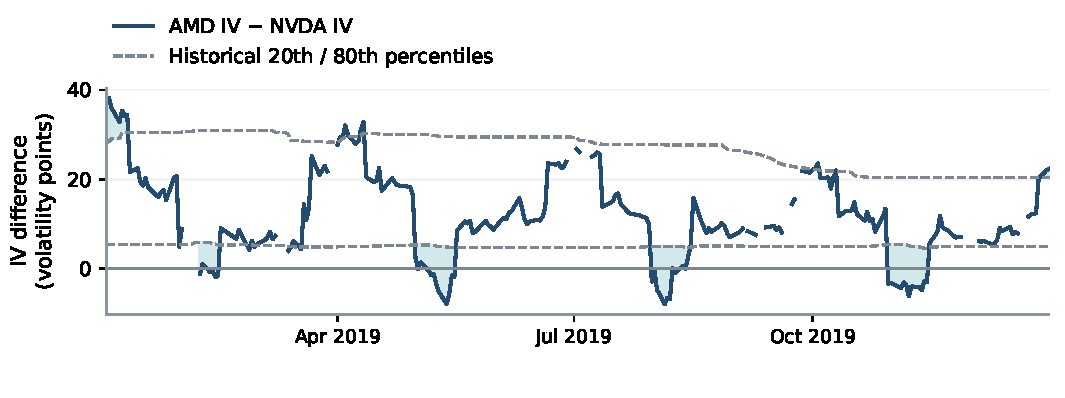
\includegraphics[width=\linewidth]{signal_example.pdf}
\caption{AMD minus NVDA selected-put IV in 2019. Shading marks excursions outside historical percentile boundaries, not executed trades. Gaps are unavailable quotes. Daily contract selection makes this a signal series, not the mark of one held contract.}\label{fig:signal-example}
\end{figure}

Monthly formation requires 126-session return beta between 0.85 and 1.15 and correlation of at least 0.5. The proposed direction must also show positive historical profit per initial vega over 91 and 365 calendar days, with 21 and 63 completed observations. These are simulated standalone candidates, not just funded fills. A trade entered yesterday with a month left cannot contribute its eventual profit today.


\subsection{Relatedness and Profitability Filters}

Beta measures the scale of one name's response to the other; correlation measures how consistently they move together. Neither guarantees that their option prices should behave alike. The relatedness screens keep the comparison among reasonably similar names without treating relatedness as the trading signal.


The profitability memory adds a different economic question: has this direction recently paid for the premium and hedging costs? We are looking for an unusually wide IV difference in a direction with evidence of structural relative richness, rather than assuming every large gap must revert. The memory and completed-count conditions are selected rules, shared across all put sizing controls.


The chart follows each day's selected contract. After entry, the simulator holds the purchased and sold contracts rather than replacing them when daily selection changes. Profit therefore depends on their realized option and hedge cash flows. A temporary narrowing of the displayed IV gap is neither required nor sufficient for a profitable expiry trade.


Entry sizing uses a regression-tree context and cross-entropy policy search. The shared sizing framework is presented in Section~\ref{sec:11}; joint performance and interpretation follow in Section~\ref{sec:results}.
\FloatBarrier

\section{ATM Straddle Strategy}\label{sec:5}

The straddle strategy sells approximately 30-day ATM straddles on underlyings with the lowest completed realized-minus-implied volatility (RV--IV) memories. The signal follows the volatility-premium motivation of Goyal and Saretto \cite{goyal2009}; our experiments evaluate entry sizing and capital allocation around this fixed trading rule.


\subsection{Trading Rules and Position Construction}

For every historical candidate, subtract entry ATM-call IV from the annualized RV measured after the next-session entry close through that contract's expiry. Only after the outcome finishes can it join the signal history. Average those completed RV - IV observations over the preceding 365 calendar days, requiring 126. Rank eligible names each day and sell the bottom 10\%.


\begin{equation*}M_{i,t}=\operatorname{mean}_{u:\,t-365<T_u<t}\left(RV_{i,u\to T_u}-IV^{\rm ATM\ call}_{i,u}\right).\end{equation*}

Selection uses the cross-sectional bottom decile of eligible completed-outcome memories, without an absolute volatility-gap threshold.



Each position sells an ATM call and put with the same underlying, strike and expiry, with daily stock-delta rebalancing. Full size targets \$450 combined call-and-put vega per IV point. The portfolio retains net short-gamma and short-vega exposure, including jump and volatility-revaluation risk.




The ranking uses ATM-call IV and annualized RV in volatility units, while execution uses the complete straddle. Profit is measured from the option-and-hedge ledger after costs and financing; the RV--IV ranking is neither a variance difference nor a profit identity.




\subsection{Ridge-Based Contexts}\label{sec:straddle-sizing}

The straddle sizing model fits a 60-month ridge model to completed full-size profit, using 14 inputs and requiring 128 examples. The inputs include IV, RV-IV memory, VIX and a separate fixed-half paper portfolio's recent performance. Score terciles define three contexts. Training uses only completed straddle outcomes and does not use the Q-allocation reward.

Training examples combine predetermined date-and-rank sampling of proposals with additional proposals admitted by a separate fixed-half benchmark portfolio. Only completed outcomes with finite reward labels enter fitting: 4,116 rewards are available in the saved sample. The fitted sizing policy is applied to all 35,774 proposals; future payoff availability does not restrict live proposals.

\subsection{Position-Size Selection}\label{sec:straddle-size-map}

Each context receives 50\%, 75\% or 100\% exposure. We enumerate all 27 context-to-size maps and retain the highest Sharpe on their aggregate completed daily straddle-profit paths, including overlapping positions. Insufficient history uses half size. The context-to-size map need not increase monotonically with the ridge score because selection maximizes completed-path Sharpe. Section~\ref{app:entry-optimization} provides exact fitting details. Feature-usage and admission diagnostics follow in Section~\ref{sec:straddle-results}.

\subsection{Results}\label{sec:straddle-results}

\subsubsection{Performance}

\begin{table}[H]\centering\small
\caption{Straddle entry-sizing policies in validation and later evaluation. S denotes annualized excess Sharpe; later profit is profit above cash.}\label{tab:straddle-entry-results}
\setlength{\tabcolsep}{4pt}\renewcommand{\arraystretch}{1.18}
\begin{tabularx}{\textwidth}{@{}>{\hsize=1.66992\hsize\linewidth=\hsize\raggedright\arraybackslash}X>{\hsize=0.81055\hsize\linewidth=\hsize\raggedleft\arraybackslash}X>{\hsize=0.81055\hsize\linewidth=\hsize\raggedleft\arraybackslash}X>{\hsize=0.73242\hsize\linewidth=\hsize\raggedleft\arraybackslash}X>{\hsize=0.97656\hsize\linewidth=\hsize\raggedleft\arraybackslash}X@{}}\toprule
\textbf{Entry policy} & \textbf{2018--21 S} & \textbf{2022--25 S} & \textbf{Later entries} & \textbf{Later profit}\\\midrule
Straddle \(\cdot\) 50\% & 0.740 & 0.920 & 1782 & \$1.824m\\
Straddle \(\cdot\) 75\% & 0.542 & 0.968 & 1222 & \$2.010m\\
Straddle \(\cdot\) 100\% & 0.528 & 0.990 & 940 & \$2.206m\\
Straddle \(\cdot\) Learned sizing & 0.775 & 1.041 & 1204 & \$2.379m\\
\bottomrule\end{tabularx}\end{table}

\begin{figure}[H]\centering
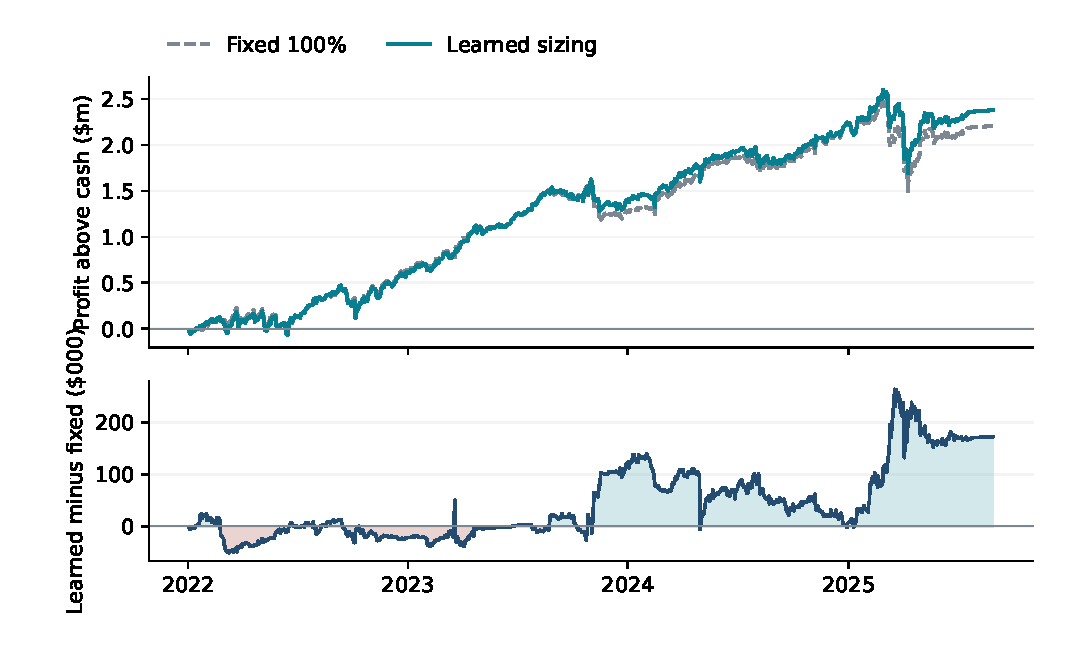
\includegraphics[width=\linewidth]{straddle_entry_curves.pdf}
\caption{Straddle profit above cash since January 2022. Top: learned and fixed-full entry sizing. Bottom: incremental profit, learned sizing minus fixed full sizing. Series subtract their 2021 closing values and retain carried positions. Differences reflect both sizing and admission.}\label{fig:straddle-entry-curves}
\end{figure}


The learned straddle sizing policy reaches Sharpe 1.041 and \$2.379 million above cash, compared with 0.990 and \$2.206 million at full size. Its earlier Sharpe also exceeds each fixed-size control.

As specified in Section~\ref{sec:evaluation-protocol}, all policies receive the same 35,774 straddle proposals, but size-dependent rounding, inventory and admission produce different funded entries. These comparisons measure complete sizing and admission policies rather than predictive sizing alone.

\subsubsection{Policy Interpretation and Trade Admission}

\begin{figure}[H]\centering
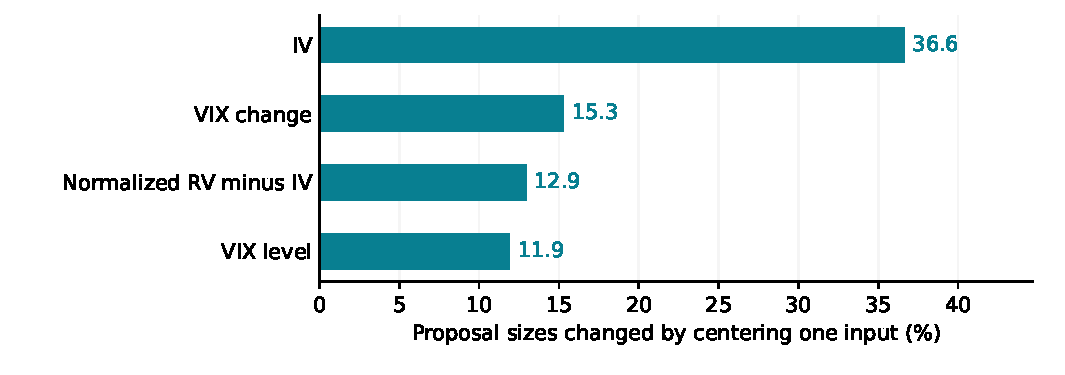
\includegraphics[width=\linewidth]{straddle_entry_explanations.pdf}
\caption{Straddle sizing sensitivity during later evaluation: the percentage of fitted proposal sizes that change when one input is centered. This descriptive sensitivity measure does not establish a causal effect on profit.}\label{fig:straddle-entry-explanations}
\end{figure}

For a straddle proposal, standardized ridge contributions add to a score. Saved thresholds locate its context, and the learned map selects a size. Centering IV changes 36.6\% of later fitted proposal sizes. Recent VIX change changes 15.3\%, normalized RV-minus-IV memory 12.9\%, and VIX level 11.9\%. The size map need not rise monotonically with the regression score because it optimizes the combined daily path. Exact replay reproduces every saved size across all 35,774 straddle proposals.

Later entry overlap with the fixed-full portfolio comprises 897 entries taken by both policies, 307 taken only by learned sizing and 43 taken only by fixed full size. These differences can arise through the inventory left by earlier size decisions. An explanation of proposed size alone therefore does not explain the entire portfolio result.

Among quote-available completed straddle labels, full-size profit averages \$1,631 for proposals assigned full size and \$16 for those assigned half size. This deliberately sampled subset also reflects admission by the fixed-half benchmark and finite-label availability; it is not a representative sample of all proposals. Three within-date size shuffles yield later Sharpes 0.834, 0.928 and 1.044, versus 1.041 learned. One shuffle exceeds the learned policy, so the funded results and feature-usage diagnostics alone do not establish predictive sizing.

Completed-cohort attribution is consistent with collecting a premium for movement risk. For both more persistent and more reversing price paths, aggregate option-plus-hedge profit is positive when entry straddle IV exceeds subsequent RV and negative when it does not. These groups use realized outcomes and are not available entry screens. There are 220 losing cohorts even when entry IV exceeds subsequent RV. Option and stock-hedge profits must be read together; positive hedge profit is not an independent trading edge. Appendix~\ref{app:h} retains the full-history attribution, IV--RV definitions and accounting reconciliation.

Joint sizing-and-allocation results follow in Section~\ref{sec:results}.
\FloatBarrier

\section{Learning Methods}\label{sec:allocation}

\subsection{Q-Learning for Capital Allocation}\label{sec:14}

The outer learner combines the funded strategy portfolios under fixed or learned entry sizing. Section~\ref{sec:11} explains the shared entry-sizing procedure. It makes a different decision: what fraction of one \$10 million budget should track each funded strategy? Its seven put/straddle targets are 100/0, 90/10, 75/25, 50/50, 25/75, 10/90 and 0/100. Weights sum to one; there is no outer leverage or cash action. A weekly decision based on prior-close information takes effect at the next close. The first session retains old holdings, then positions resize and drift until the next decision.


\subsubsection*{State and Action Spaces}

Nine state inputs describe four economic opportunities---put-spread rank strength, the put implied-versus-realized variance gap, straddle IV-versus-RV richness and completed straddle premium---plus relative strategy volatility, strategy-return correlation, VIX, relative recent Sharpe and previous straddle weight. Previous holdings matter because changing allocations incurs additional costs. A target is a fractional claim on a funded strategy index, not a new integer-contract order book. Underlying trading costs remain embedded in source returns; resizing adds source-based option and hedge charges.


\begin{equation*}R_w(\lambda)=\sum_{d\in w}(z_d-\lambda z_d^2),\qquad z_d=e_d/\widehat{\sigma}_{\mathrm{ref}}\end{equation*}

\subsubsection*{Reward Specification and Fitted Q Iteration}

Reference volatility is estimated from the training window's fixed-50/50 excess returns. The parameter \(\lambda\) penalizes squared normalized fluctuations. At \(\lambda\) = 0, the directive is profit alone: additional normalized return earns reward without an explicit charge for the accompanying volatility. A higher-profit, higher-variance strategy can therefore attract capital even when its risk-adjusted performance is weaker. This objective does not maximize Sharpe. The discount \(\gamma\) = 0.99 separately weights continuation value; it is unchanged across risk preferences.


Monthly fitted Q iteration uses the preceding 104 completed weeks, with at least 52. A quadratic function of straddle weight has coefficients linear in standardized state, giving 30 coefficients. Each Bellman update regresses immediate reward plus discounted next-state maximum value onto the same basis \cite{ernst2005}. We use ridge coefficient 10 and 200 updates. Seven prior allocations crossed with seven actions supply counterfactual paths on each market week; they do not create independent market observations.


Q uses 50/50 before enough training weeks exist; each fixed control starts at its own target. A discount-zero learner supplies a matched one-period control. In the factorial experiment, Q is refitted independently for each entry policy. Strategy-dependent risk features, reward paths and resizing charges are rebuilt for that policy, while economic signal definitions remain shared.


The outer experiment holds each signal's proposals fixed while learning how to combine their exposures. Entry sizes change the inner funded portfolios; Q changes the capital assigned across them. The accounting layers are deliberately distinct, allowing us to remove either learning layer in the four-way comparison.


\FloatBarrier
\subsection{Contextual Bandit Entry Sizing}\label{sec:11}

We use direct policy search to learn a contextual sizing policy that maximizes historical portfolio Sharpe. The rule fixes direction and contracts; the bandit chooses 50\%, 75\% or 100\% exposure. CEM optimizes the put policy.


\subsubsection*{Regression Tree and Cross-Entropy Policy Search}

Each monthly regression tree uses completed examples from the preceding 18 months. Its target is cumulative full-size profit above cash; splits reduce prediction error across 27 inputs. At most eight leaves define states. With n examples, minimum leaf count is max(8, min(63, floor(n/8))); fewer than 16 use full size.


\begin{figure}[!htbp]\centering
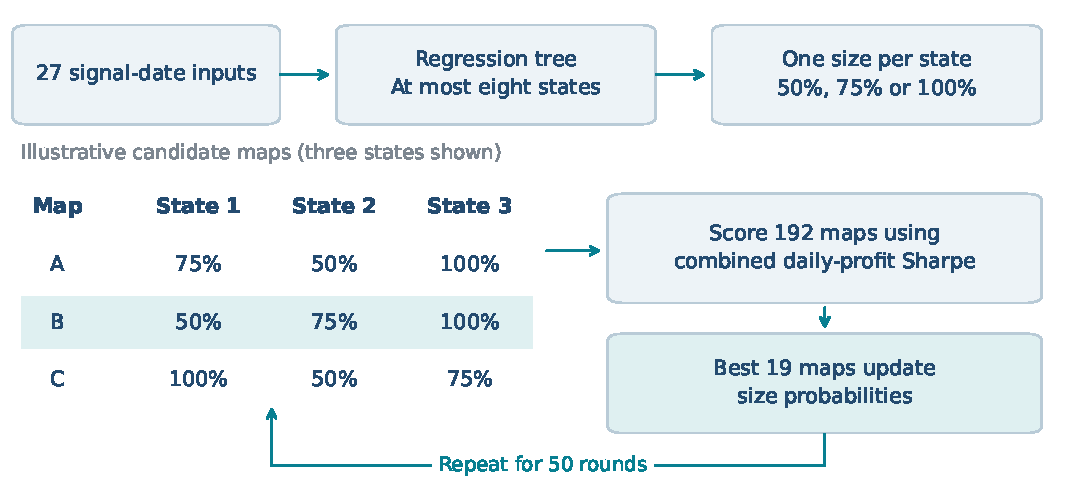
\includegraphics[width=\linewidth]{entry_policy.pdf}
\caption{The original tree/CEM construction. The three-state maps illustrate candidates; actual trees have up to eight states. Each candidate selects action-specific completed paths; the best 19 update sampling probabilities. The retained map sizes next month's proposals.}\label{fig:entry-policy}
\end{figure}

For completed example i, p denotes its profit above cash on day d at size a. Each size has its own rounded contracts and simulated hedge path. A map assigns one size to each tree state. We sum its daily paths, retaining overlapping positions and zero-profit sessions, and score the result:


\begin{equation*}g_d(m)=\sum_i p_{i,d}(a_{\ell(x_i)}),\qquad\widehat S_{\rm train}(m)=\sqrt{252}\,\overline{g}/s_g.\end{equation*}

CEM \cite{deboer2005} updates size probabilities toward the best 19 of 192 candidate maps for 50 rounds. Constant maps and the incumbent are anchors. This standalone-path training score differs from funded-account Sharpe: replay additionally applies shared cash, inventory and admission.


The 27-input, 18-month specification was retained from 33 archived configurations ranked on 2018--2021 validation scores. Archived selection used a \$345 million research account; the funded comparisons below use \$10 million. Detailed feature experiments and the refitting timeline are in Appendix~\ref{app:g}; exact fitting settings are in Appendix~\ref{app:b}.

\subsubsection*{Ridge Regression and Context-Based Sizing}

The straddle bandit fits a 60-month ridge model to completed full-size profit, using 14 inputs and requiring 128 examples. The inputs include IV, RV-IV memory, VIX and a separate fixed-half paper portfolio's recent performance. Score terciles define three states. We enumerate all 27 size maps and retain the highest training Sharpe. Insufficient history uses half size. Both learners use completed outcomes; Appendix~\ref{app:b} provides exact fitting details.




The policy chooses 50\%, 75\% or 100\% exposure within the same completed-path Sharpe framework used for put pairs. The ridge score groups opportunities; the selected context-to-size map determines the requested size and need not increase monotonically with the score. The model uses completed quote-available labels: 4,116 training rewards are finite, while the policy handles all 35,774 proposals. Section~\ref{sec:13} reports feature-usage and admission diagnostics.
\FloatBarrier

\section{Discussion and Conclusion}\label{sec:20}

\subsection*{Summary of Findings}

Learned entry policies improve the retained portfolios through sizing and admission. Q improves allocation with constant entries and exceeds the corresponding rolling mean--variance controls at \(\lambda\) = 0.10, 0.20 and 1. Its profit-only policy transfers less reliably when straddles weaken. These are illustrative risk-preference comparisons. The original validation-selected \(\lambda=0.025\) policy falls from validation Sharpe 1.437 to later Sharpe 0.282, so validation-based policy selection did not transfer its strong historical performance. Reward design changes the allocation tradeoff.


\subsection*{Limitations}

All fitted policies use only information available before their decisions. However, the extent to which later-period inspection influenced development, including training-window and risk-preference choices, remains to be verified (Section~\ref{app:research-chronology}). The evaluation should therefore be interpreted as historical performance under chronologically fitted policies, rather than a confirmed independently frozen test of the complete research process. The controlled comparisons provide evidence about adaptive exposure allocation under the stated assumptions, but neither the magnitude of research-selection bias nor prospective performance has been established.


Execution is another boundary. Midpoint-based fills with an adverse charge do not establish tradability, particularly for paired orders that may fill asynchronously. Quoted-spread execution, liquidity capacity, pin risk, early assignment and forced liquidation need further work. The outer experiment reallocates fractional strategy indices, not shared integer contracts. Initial vega matching is local, and the straddle signal adds net short-volatility risk.


\Needspace{15\baselineskip}

\subsection*{Conclusion}

The experiments support adaptive exposure allocation across portfolios with different capital deployment and volatility risks. The four-way comparison separates entry learning from allocation, while the dynamic benchmarks and one-period control place the Q result in context. The evidence is strongest for conditional allocation under the stated historical simulation assumptions; policy rankings depend on the profit--risk objective, and the original validation-selected policy performs weakly in the later period. The headline illustrative policy therefore does not establish successful validation-based selection or prospective performance.

Appendix~\ref{app:h} relates straddle profitability to realized movement. An integrated implementation should combine entry sizing, allocation and inventory controls under measured execution costs, followed by prospective evaluation and tests on additional independent signals.


\FloatBarrier


\bibliographystyle{unsrtnat}
\bibliography{references}
\clearpage
\appendix
\begingroup
\renewcommand{\baselinestretch}{1}
\fontsize{10.5}{12.8}\selectfont
\clearpage
\section{Contract Selection, Features, and Risk Constraints}\label{app:a}

This appendix separates contract selection, the inputs to each strategy's sizing model, and the admission rules used in the funded contract-level replays. Allocation-state inputs are defined separately in Section~\ref{sec:allocation}.

\subsection{Data and Contract Selection}\label{app:contracts}

The data universe and coverage limitations are described in Section~\ref{sec:data}. Table~\ref{tab:contract-selection} distinguishes the two contract screens.

\begin{table}[H]\centering\small
\caption{Strategy-specific contract selection.}\label{tab:contract-selection}
\setlength{\tabcolsep}{5pt}\renewcommand{\arraystretch}{1.2}
\begin{tabularx}{\textwidth}{@{}>{\hsize=.55\hsize\linewidth=\hsize\raggedright\arraybackslash}X>{\hsize=1.225\hsize\linewidth=\hsize\raggedright\arraybackslash}X>{\hsize=1.225\hsize\linewidth=\hsize\raggedright\arraybackslash}X@{}}\toprule
\textbf{Criterion} & \textbf{Put pair} & \textbf{Straddle}\\\midrule
Expiry & Nearest 30 days; entry requires 7--55 days remaining & ATM-call signal screen requires 21--45 days from next-session entry to expiry\\[4pt]
Strike or delta & Put nearest absolute delta 0.25, within 0.075 & ATM-call strike within 10\% of spot\\[4pt]
Position legs & Selected put on each related underlying & Call and put match on underlying, strike, expiry and adjustment\\
\bottomrule\end{tabularx}\end{table}

Both screens require standard 100-share contracts, positive noncrossed quotes, open interest of at least 100 and quote width no more than 25\% of midpoint. Put-selection ties prefer narrower quotes, higher open interest and then lower contract identifier.

\paragraph{Quote handling and valuation}
Missing entry quotes reject proposals. Corporate events can force exits. Held marks may use last-known IV with current spot, rates and known dividends. European-style valuation and cash settlement approximate expiry; assignment is not fully simulated.

\subsection{Put-Pair Sizing Inputs}\label{app:features}

The tree uses 15 numerical inputs and 12 binary availability flags, giving 27 inputs in total. In Table~\ref{tab:put-sizing-inputs}, starred inputs are required; every other numerical input has an availability flag.

\begingroup\small
\setlength{\tabcolsep}{4pt}\renewcommand{\arraystretch}{1.15}
\begin{longtable}{@{}>{\raggedright\arraybackslash}p{0.32\textwidth}>{\raggedright\arraybackslash}p{\dimexpr0.68\textwidth-8pt\relax}@{}}
\caption{Numerical inputs to put-pair sizing; starred inputs are required.}\label{tab:put-sizing-inputs}\\
\toprule\textbf{Input} & \textbf{Definition}\\\midrule
\endfirsthead
\multicolumn{2}{l}{\textit{Put-pair sizing inputs (continued)}}\\
\toprule\textbf{Input} & \textbf{Definition}\\\midrule
\endhead
\midrule\multicolumn{2}{r}{\textit{Continued on next page}}\\\endfoot
\bottomrule\endlastfoot
\multicolumn{2}{l}{\textit{Signal and volatility}}\\*[3pt]
Mean IV\textsuperscript{*} & Mean implied volatility of the selected puts\\[3pt]
Directional IV gap\textsuperscript{*} & IV gap oriented to the proposed trade direction\\[3pt]
Spread-rank strength\textsuperscript{*} & Strength of the historical IV-spread rank signal\\[3pt]
Directional variance gap & Oriented IV-squared minus trailing-variance gap\\[3pt]
Mean realized volatility & Mean trailing stock realized volatility\\[3pt]
\multicolumn{2}{l}{\textit{Pair relatedness}}\\*[3pt]
Return beta & 126-session stock-return beta\\[3pt]
Return correlation & 126-session stock-return correlation\\[3pt]
\multicolumn{2}{l}{\textit{Contract terms and costs}}\\*[3pt]
Mean time to expiry & Mean days remaining to expiry\\[3pt]
Directional expiry gap & Expiry difference oriented to trade direction\\[3pt]
Commission relative to vega & Training commission expressed in IV points\\[3pt]
\multicolumn{2}{l}{\textit{Market conditions}}\\*[3pt]
VIX & Strictly prior VIX close\\[3pt]
\multicolumn{2}{l}{\textit{Completed directional outcomes}}\\*[3pt]
91-day profitability & Mean completed profit per initial vega over 91 calendar days\\[3pt]
91-day observation count & Number of completed observations in that window\\[3pt]
365-day profitability & Mean completed profit per initial vega over 365 calendar days\\[3pt]
365-day observation count & Number of completed observations in that window\\[3pt]
\end{longtable}\endgroup

An availability flag is one when its numerical field is observed and zero otherwise. Missing optional values are set to zero with flag zero; an observed numerical zero retains flag one. Put trailing variance is 252 times mean squared simple stock returns over 20 sessions, requiring at least ten observations.

\subsection{Straddle Sizing Inputs}\label{app:straddle-features}

The ridge model uses the 14 inputs in Table~\ref{tab:straddle-sizing-inputs}. Benchmark features come from a separate fixed-half straddle portfolio constructed using information available at each date, not the learner's future inventory.

\begingroup\small
\setlength{\tabcolsep}{4pt}\renewcommand{\arraystretch}{1.15}
\begin{longtable}{@{}>{\raggedright\arraybackslash}p{0.34\textwidth}>{\raggedright\arraybackslash}p{\dimexpr0.66\textwidth-8pt\relax}@{}}
\caption{All 14 inputs to the retained straddle ridge model.}\label{tab:straddle-sizing-inputs}\\
\toprule\textbf{Input} & \textbf{Definition}\\\midrule
\endfirsthead
\multicolumn{2}{l}{\textit{Straddle sizing inputs (continued)}}\\
\toprule\textbf{Input} & \textbf{Definition}\\\midrule
\endhead
\midrule\multicolumn{2}{r}{\textit{Continued on next page}}\\\endfoot
\bottomrule\endlastfoot
\multicolumn{2}{l}{\textit{Volatility opportunity and recent changes}}\\[3pt]
Completed RV--IV memory & Historical completed realized-minus-implied volatility memory from Section~\ref{sec:5}\\[3pt]
IV & Current ATM-call implied volatility\\[3pt]
VIX & VIX level available at the proposal date\\[3pt]
Normalized memory & Negative RV--IV memory divided by current IV, with IV floored at 0.01\\[3pt]
Variance ratio & Forecast annualized variance divided by squared IV\\[3pt]
21-session VIX change & Proportional change in VIX over 21 sessions\\[3pt]
5-session IV change & Proportional change in IV over five sessions\\[3pt]
\multicolumn{2}{l}{\textit{Fixed-half benchmark portfolio}}\\[3pt]
21-session Sharpe & Annualized excess Sharpe over 21 sessions\\[3pt]
63-session Sharpe & Annualized excess Sharpe over 63 sessions\\[3pt]
126-session Sharpe & Annualized excess Sharpe over 126 sessions\\[3pt]
63-session volatility & Annualized daily excess-return volatility over 63 sessions\\[3pt]
63-session drawdown & Cash-relative wealth divided by its trailing 63-session maximum, minus one\\[3pt]
Reserve use & Capital reserve divided by current portfolio NAV\\[3pt]
Benchmark availability & Binary flag indicating that the benchmark features are available\\[3pt]
\end{longtable}\endgroup

\subsection{Risk Limits and Admission}\label{app:risk}

The limits in Table~\ref{tab:admission-risk-limits} govern funded contract-level admission, not the outer strategy-index allocation.

\begin{table}[H]\centering\small
\caption{Risk limits used in contract-level admission checks.}\label{tab:admission-risk-limits}
\setlength{\tabcolsep}{5pt}\renewcommand{\arraystretch}{1.25}
\begin{tabularx}{\textwidth}{@{}>{\hsize=.65\hsize\linewidth=\hsize\raggedright\arraybackslash}X>{\hsize=1.35\hsize\linewidth=\hsize\raggedright\arraybackslash}X@{}}\toprule
\textbf{Check} & \textbf{Limit or definition}\\\midrule
Stress loss & At most 5\% of the applicable budget\\[3pt]
Capital reserve & At most 80\% of the applicable budget\\[3pt]
Hedge notional & At most twice the applicable budget\\[3pt]
Gross vega & At most \$20,000 per IV point per \$1 million of reference capital\\[3pt]
Reserve measurement & Gross option premium plus half the netted hedge notional\\[3pt]
Budget scope & Global checks use equity; pair checks use a \$1 million reference scaled by current divided by initial equity\\
\bottomrule\end{tabularx}\end{table}

Stress testing takes each name's worst modeled option-plus-hedge loss across spot shocks of \(-20\%,0,+20\%\) and IV shocks of \(-10,0,+10\) points. These losses are summed without pair-correlation credit. Quote eligibility, inventory and the limits above jointly determine whether a proposed size is admitted.

\FloatBarrier

\subsection{Data and Code Availability}\label{app:reproduction}

Supporting materials, saved results and figures are available at \url{https://github.com/kreitzz/rl-atm-vega-pairs}. Access to the underlying WRDS data requires the relevant subscriptions and vendor permissions; redistribution restrictions apply. Model fitting requires the licensed source cache or suitable archived derived inputs.

Public snapshots support reproduction of the attribution and associated figures from saved derived data, without raw option chains. This verifies archived results rather than independently refitting the models or regenerating all trading experiments. Source locations, verification details and reproduction guidance are provided in the paper's repository README.
\FloatBarrier

\clearpage
\section{Model Estimation and Selection}\label{app:b}\label{app:g}
This appendix records feature selection, fitting conventions and research chronology for the strategy-specific sizing policies and the capital allocator.

\subsection{Feature and Model Selection}\label{app:feature-selection}\label{sec:10}

Section~\ref{app:features} lists the 27 retained put inputs and their availability conventions. Future trade profits serve as training outcomes, never current inputs.


\subsubsection*{Variance Premium Features}

One additional block compares squared IV with forecast annualized variance. Its forecast uses exponentially weighted squared daily returns, with a 20-session half-life and at least 63 observations. Multiplication by 252 annualizes the estimate. The block adds the spread, a historical z-score and forecast-to-implied variance ratio, with availability flags.


\begin{equation*}\text{Variance spread}=IV^2-\widehat{\sigma}_{\rm RV}^{\,2}.\end{equation*}

IV and forecast volatility enter in decimal units, so the spread is a variance difference. Downside-put skew prevents interpreting it as a clean underlying variance-risk-premium estimate. The EWMA block is a tested addition; it is not part of the retained 27-input put baseline.


\begin{figure}[H]\centering
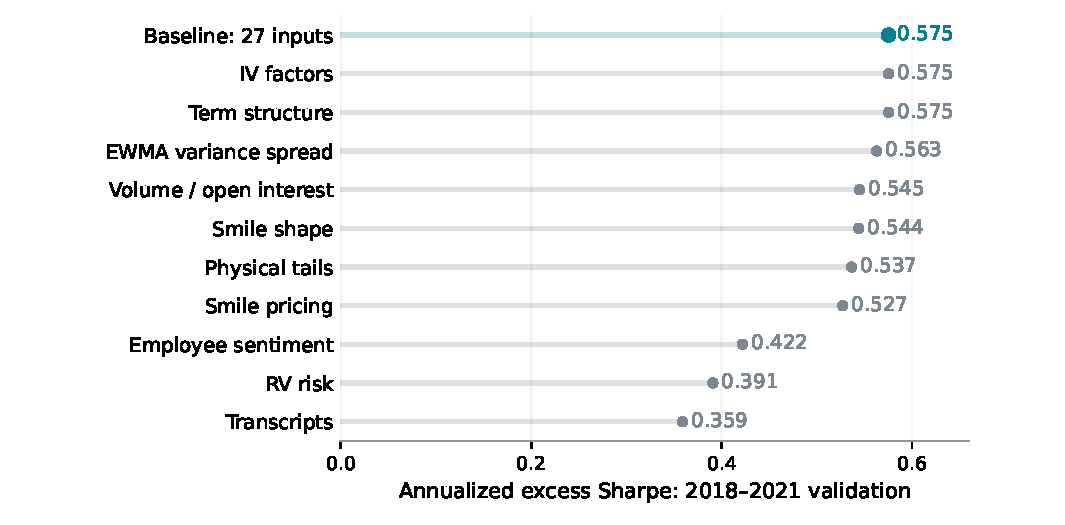
\includegraphics[width=\linewidth]{feature_validation.pdf}
\caption{Original feature exploration at the 18-month baseline. Scores use 2018--2021 validation and the archived \$345 million research account; funded policy comparisons use \$10 million. The three highest scores tie exactly.}\label{fig:feature-validation}
\end{figure}

We rank 33 archived screened configurations by 2018--2021 validation excess Sharpe within the established 30-day, 25-delta design. Feature, window and action-menu experiments form this grid. Baseline, IV-factor and term-structure scores tie exactly at 0.575; alphabetical configuration ordering retains the baseline. The selected specification has 27 inputs, an 18-month window and 50/75/100\% sizes.


Archived selection scores use a \$345 million research account; funded replays use \$10 million. This split selects the sizing procedure within the established contract design and pair roster. Section~\ref{app:research-chronology} records extension selection histories.


\FloatBarrier

\subsection{Monthly Refitting Timeline}\label{app:refitting-timeline}

\begin{figure}[!htbp]\centering
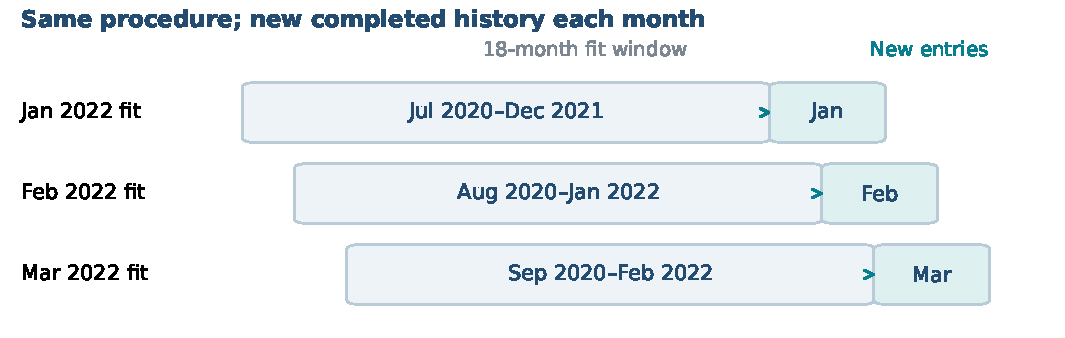
\includegraphics[width=\linewidth]{refit_timeline.pdf}
\caption{Monthly put-policy refitting. Only completed outcomes whose signal dates fall in the displayed 18-month window enter each fit. The selected model settings remain fixed; the tree and size assignments update.}\label{fig:refit-timeline}
\end{figure}


\FloatBarrier

\subsection{Entry Policy Optimization}\label{app:entry-optimization}

Put entry sizing follows Section~\ref{sec:11}. CEM uses 50 rounds of 192 maps, 19 elites and seed 2026. Probabilities start uniform; updates mix 30\% prior probability and 70\% elite frequency, shrink by 0.97 and add 0.03 uniformly. Constant maps and the incumbent are anchors. Separate rounded-contract paths supply daily training profits; funded NAV returns supply evaluation Sharpe. Put memory and training labels retain a \$0.65 option commission; funded evaluation uses \$0.03 for every policy.


The straddle ridge fit uses median centers, standard deviations floored at 0.001, clipped inputs within \(\pm\)5, penalty 100 with no intercept penalty, and equal total weight per date. Full-size completed profit is its target. Score terciles define contexts; all 27 size maps are evaluated on aggregate daily paths. Ties favor lower exposure. The 60-month window requires 128 examples. Only 4,116 training rewards are finite; the policy still handles all 35,774 proposals.



\subsection{Q-Function Specification and Convergence}\label{app:q-convergence}


The Q-function basis, state normalization, ridge penalties and weekly regression weighting are specified in Section~\ref{sec:allocation}. All 81 monthly fits were checked at 200, 500, 1,000 and 2,000 updates. Later actions are identical across budgets for the four reported \(\lambda\) values.



\FloatBarrier
\subsection{Research Chronology and Statistical Inference}\label{app:research-chronology}
Every fit uses strictly completed past outcomes. Put selection ranks 33 archived screened configurations by 2018--2021 scores before the \$10 million replay. The straddle's 48- and 60-month windows tie at validation Sharpe 0.775; later Sharpes of 0.960 and 1.041 informed refinement. The four displayed Q preferences illustrate researched risk choices, not a single validation-winning policy. The original selection and full results remain in \path{reports/signal_allocation_discount}. The put-sizing gain is 0.208, with a paired 95\% interval of -0.103 to +0.424, using 1,000 circular resamples of 126-session blocks, fixed policies and no selection adjustment. These records identify research choices without measuring their bias.
\FloatBarrier

\clearpage
\section{Supplementary Results and Diagnostics}\label{app:c}\label{app:d}\label{app:e}
The tables and diagnostics below supplement the main policy comparisons. Reporting measures are defined in Section~\ref{sec:performance-measures}.

\subsection{Annual Performance and Reward Sensitivity}\label{app:annual-results}
\begin{table}[H]\centering\small
\caption{Annualized excess Sharpe by calendar year; 2025 ends in August.}
\setlength{\tabcolsep}{4pt}\renewcommand{\arraystretch}{1.18}
\begin{tabularx}{\textwidth}{@{}>{\hsize=0.68359\hsize\linewidth=\hsize\raggedright\arraybackslash}X>{\hsize=1.07422\hsize\linewidth=\hsize\raggedleft\arraybackslash}X>{\hsize=1.07422\hsize\linewidth=\hsize\raggedleft\arraybackslash}X>{\hsize=1.07422\hsize\linewidth=\hsize\raggedleft\arraybackslash}X>{\hsize=1.09375\hsize\linewidth=\hsize\raggedleft\arraybackslash}X@{}}\toprule
\textbf{Year} & \textbf{Put bandit} & \textbf{Straddle bandit} & \textbf{Q: \(\lambda\) = .20} & \textbf{Q: \(\lambda\) = 1}\\\midrule
2018 & 0.522 & 0.148 & 0.160 & 0.160\\
2019 & -0.542 & 1.459 & 0.112 & -0.237\\
2020 & 1.555 & 0.161 & 1.617 & 1.028\\
2021 & -0.580 & 2.336 & 2.932 & 3.180\\
2022 & 2.458 & 1.206 & 2.042 & 2.540\\
2023 & 1.492 & 1.727 & 2.449 & 2.907\\
2024 & -0.907 & 1.465 & 1.945 & 1.954\\
2025* & 1.092 & 0.085 & -0.598 & 1.092\\
\bottomrule\end{tabularx}\end{table}

All figures are annualized excess Sharpe; 2025 ends on 29 August. The sleeves retain their separate funded histories, and outer allocations include resizing charges. Annual results show substantial regime variation.


\begin{table}[H]\centering\small
\caption{Later excess Sharpe across entry policies and Q reward preferences.}
\setlength{\tabcolsep}{4pt}\renewcommand{\arraystretch}{1.18}
\begin{tabularx}{\textwidth}{@{}>{\hsize=1.48438\hsize\linewidth=\hsize\raggedright\arraybackslash}X>{\hsize=0.87891\hsize\linewidth=\hsize\raggedleft\arraybackslash}X>{\hsize=0.87891\hsize\linewidth=\hsize\raggedleft\arraybackslash}X>{\hsize=0.87891\hsize\linewidth=\hsize\raggedleft\arraybackslash}X>{\hsize=0.87891\hsize\linewidth=\hsize\raggedleft\arraybackslash}X@{}}\toprule
\textbf{Entry policy + Q} & \textbf{\(\lambda\) = 0} & \textbf{\(\lambda\) = .10} & \textbf{\(\lambda\) = .20} & \textbf{\(\lambda\) = 1}\\\midrule
Fixed 50\% & 0.541 & 0.703 & 1.116 & 1.349\\
Fixed 75\% & 0.606 & 0.667 & 2.118 & 1.897\\
Fixed 100\% & 0.618 & 1.354 & 1.194 & 1.633\\
Bandit & 0.671 & 1.491 & 1.726 & 2.152\\
\bottomrule\end{tabularx}\end{table}

This table holds Q's feature definitions, discount, training window and action menu fixed while refitting separately on each entry family. Values are 2022--2025 Sharpes. The complete seven fixed capital splits are also retained; 50/50 is the primary fixed-allocation baseline, rather than a later-period optimized control.
\FloatBarrier
\subsection{Additional Put-Sizing Results}\label{app:additional-put-results}
\begin{table}[H]\centering\small
\caption{Alternative put-sizing policies on the common reporting split.}
\setlength{\tabcolsep}{4pt}\renewcommand{\arraystretch}{1.18}
\begin{tabularx}{\textwidth}{@{}>{\hsize=1.75781\hsize\linewidth=\hsize\raggedright\arraybackslash}X>{\hsize=0.78125\hsize\linewidth=\hsize\raggedleft\arraybackslash}X>{\hsize=0.78125\hsize\linewidth=\hsize\raggedleft\arraybackslash}X>{\hsize=0.70312\hsize\linewidth=\hsize\raggedleft\arraybackslash}X>{\hsize=0.97656\hsize\linewidth=\hsize\raggedleft\arraybackslash}X@{}}\toprule
\textbf{Put sizing policy} & \textbf{2018--21 S} & \textbf{2022--25 S} & \textbf{Later entries} & \textbf{Later profit}\\\midrule
Constant 50\% & 0.437 & 1.007 & 151 & \$0.205m\\
Constant 75\% & 0.449 & 0.944 & 104 & \$0.195m\\
Constant 100\% & 0.478 & 1.055 & 75 & \$0.201m\\
Tree + CEM & 0.573 & 1.263 & 110 & \$0.249m\\
Spread-rank sizing & 0.464 & 0.815 & 121 & \$0.165m\\
Ridge-score sizing & 0.421 & 0.890 & 94 & \$0.180m\\
Direct linear policy & 0.267 & 0.873 & 96 & \$0.171m\\
Direct additive policy & 0.302 & 1.013 & 97 & \$0.180m\\
\bottomrule\end{tabularx}\end{table}

All policies receive the same put proposals, directions, contracts and funded admission rules. The lower four rows are follow-up comparisons rather than original selection candidates. Tree/CEM has the highest funded Sharpe in both periods among these policies. These comparisons retain the original question about entry sizing alongside the newer straddle and allocation experiments.


\begin{table}[H]\centering\small
\caption{Put-bandit annual account returns and excess performance.}
\setlength{\tabcolsep}{4pt}\renewcommand{\arraystretch}{1.18}
\begin{tabularx}{\textwidth}{@{}>{\hsize=0.58594\hsize\linewidth=\hsize\raggedright\arraybackslash}X>{\hsize=1.07422\hsize\linewidth=\hsize\raggedleft\arraybackslash}X>{\hsize=1.22070\hsize\linewidth=\hsize\raggedleft\arraybackslash}X>{\hsize=1.17188\hsize\linewidth=\hsize\raggedleft\arraybackslash}X>{\hsize=0.94727\hsize\linewidth=\hsize\raggedleft\arraybackslash}X@{}}\toprule
\textbf{Year} & \textbf{Account return} & \textbf{Above cash (pp)} & \textbf{Excess Sharpe} & \textbf{Entries}\\\midrule
2022 & 3.470\% & 1.673 & 2.458 & 66\\
2023 & 5.288\% & 0.432 & 1.492 & 19\\
2024 & 5.104\% & -0.283 & -0.907 & 11\\
2025* & 3.207\% & 0.169 & 1.092 & 14\\
\bottomrule\end{tabularx}\end{table}

Calendar-period account returns and above-cash differences are not annualized, including partial 2025. Sharpe is annualized. In 2024 the account grows while losing relative to cash. Profit is concentrated: SNAP/UBER, GAP/TJX and AMD/MU contribute 66.9\% of later net pair trading profit, and 2022 supplies 83.1\%. These figures exclude shared financing. They describe where gains occurred, not a rule for selecting those names retrospectively. Section~\ref{app:annual-results} reports the annual Sharpe ratios.


The put account's later annualized total account return is 4.667\%, versus 0.530\% growth relative to cash. Average reserve is 2.44\% and peak reserve 15.77\%. Its cash-relative drawdown is 0.495\%, compared with 0.646\% at full size. These figures retain the original distinction between a profitable trading signal, account funding and capital deployment.
\FloatBarrier
\subsection{Allocation Timing Diagnostics}\label{app:timing}
\begin{table}[H]\centering\small
\caption{Allocation timing controls at \(\lambda\) = 0.20.}
\setlength{\tabcolsep}{4pt}\renewcommand{\arraystretch}{1.18}
\begin{tabularx}{\textwidth}{@{}>{\hsize=1.71875\hsize\linewidth=\hsize\raggedright\arraybackslash}X>{\hsize=0.75000\hsize\linewidth=\hsize\raggedleft\arraybackslash}X>{\hsize=0.75000\hsize\linewidth=\hsize\raggedleft\arraybackslash}X>{\hsize=0.78125\hsize\linewidth=\hsize\raggedleft\arraybackslash}X@{}}\toprule
\textbf{Allocation control, \(\lambda\) = .20} & \textbf{2018--21 S} & \textbf{2022--25 S} & \textbf{Later profit}\\\midrule
Fixed at Q's mean target & 0.828 & 1.387 & \$0.841m\\
One-period learner, \(\gamma\) = 0 & 1.053 & 1.645 & \$1.184m\\
Sequential Q, \(\gamma\) = 0.99 & 1.215 & 1.726 & \$1.306m\\
\bottomrule\end{tabularx}\end{table}

Centering VIX and straddle IV-versus-RV richness changes 13.6\% and 12.6\% of later actions. The mean-weight control uses Q's realized average target retrospectively. 49 nonzero circular rotations preserve allocation counts and most serial structure, then recompute wealth and resizing costs. None reaches actual later Sharpe; three reach or exceed actual validation Sharpe, and median later Sharpe is 0.744. These are descriptive information-use and timing diagnostics, without causal feature attribution or research-selection adjustment.

\FloatBarrier
\subsection{Reporting Boundaries and Account Construction}\label{app:account-boundaries}
At the 2021 close, the learned put account has \$10.568 million equity and four open trades; full sizing has \$10.581 million and three. Cash benchmark wealth is \$10.510 million. Performance curves subtract each policy's opening dollar excess wealth; they do not reset accounts or liquidate inventory at the reporting split.

A final distinction concerns portfolio admission. The source put and straddle books each simulate whole contracts and daily stock hedges under their own funded histories. The outer allocator trades fractional claims on those net strategy indices, with additional resizing charges. Its capital weights are not premium deployment or broker margin, and reallocating indices does not rerun a common integer-contract inventory ledger.
\subsection{Position Construction and Risk Accounting}\label{app:position-construction}\label{sec:3}
The following example specifies the vega units, hedge signs and residual exposures of the approximately 30-day, 25-delta put-pair construction.


\subsubsection*{Vega Matching and Delta Hedging}

Vega measures the change in option value when IV rises by one percentage point---for example, from 30\% to 31\%. The table reports total position vega; each option contract represents 100 shares. These are illustrative numbers, not an observed trade.


\begin{table}[H]\centering\small
\caption{Illustrative put pair with matched initial vega.}
\setlength{\tabcolsep}{4pt}\renewcommand{\arraystretch}{1.18}
\begin{tabularx}{\textwidth}{@{}>{\hsize=0.84375\hsize\linewidth=\hsize\raggedright\arraybackslash}X>{\hsize=0.58594\hsize\linewidth=\hsize\raggedleft\arraybackslash}X>{\hsize=1.21094\hsize\linewidth=\hsize\raggedright\arraybackslash}X>{\hsize=1.35938\hsize\linewidth=\hsize\raggedright\arraybackslash}X@{}}\toprule
\textbf{Position} & \textbf{Contracts} & \textbf{Total vega per IV point} & \textbf{Initial stock hedge}\\\midrule
Buy A puts & +100 & +\$450 & Buy 2,500 shares\\
Sell B puts & -150 & -\$450 & Short 3,750 shares\\
\bottomrule\end{tabularx}\end{table}

Each A contract has \$4.50 of vega and each B contract \$3.00. Buying 100 A contracts and selling 150 B contracts therefore balances +\$450 against -\$450. An equal one-point IV increase approximately cancels at entry. Both puts initially have delta -0.25 per share: the long puts require buying stock, while the short puts require selling it. Equal option counts would generally fail to balance vega.


If A's IV instead rises by two points while B's rises by one, the initial vega approximation gives a \$900 gain on A and a \$450 loss on B: a \$450 net gain before other effects. This is a local approximation to changes in option marks, not a formula for profit earned by holding to expiry. We match vega at entry and adjust stock delta hedges daily; we do not continuously restore vega neutrality.


With vega \(V\) and IV changes in matching volatility-point units, the local delta-hedged expansion is \(\Delta P_{\rm hedged}\approx\frac{1}{2}\Gamma(\Delta S)^2+\Theta\Delta t+V\Delta IV\).
\FloatBarrier

\clearpage
\section{Straddle Attribution and Reconciliation}\label{app:h}\label{app:f}

This appendix explains the straddle account's full-history profit, January 2018--August 2025. It supports the strategy's economic interpretation, not the incremental value of learned sizing or Q allocation.

\subsection{Straddle Profit Attribution}\label{sec:6}

Across 2,599 executed cohorts under learned sizing, options after option charges earned \$1.74 million and stock hedges before hedge costs earned \$1.75 million. Their combined \$3.49 million reconciles to \$3.75 million above cash after the remaining costs, dividends and financing, as shown below.

\begin{figure}[H]\centering
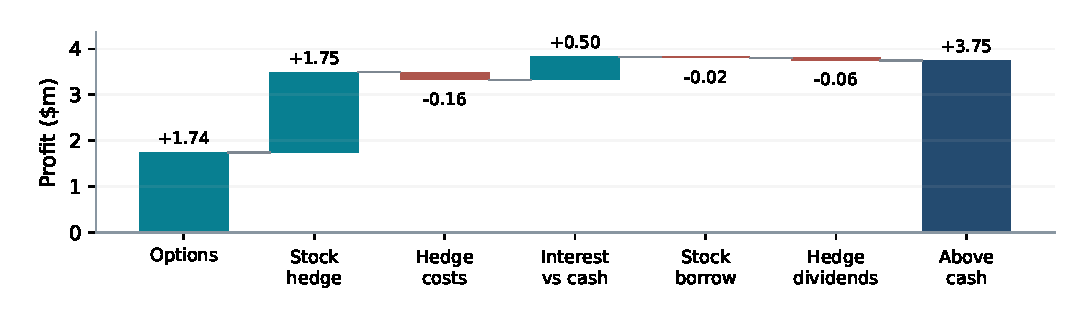
\includegraphics[width=\linewidth]{straddle_bridge.pdf}
\caption{Full-history straddle account, January 2018--August 2025. The option and stock components are read together; the remaining cash flows reconcile them to profit above cash.}\label{fig:straddle-bridge}
\end{figure}

The option and hedge components must be read together. Option marks reflect time decay, stock-price moves and volatility revaluation; the stock position offsets option delta. Positive profits in both components therefore do not establish two independent sources of alpha.

\subsection{Implied and Realized Volatility}\label{sec:7}

Table~\ref{tab:straddle-ivrv-attribution} groups the same cohorts by entry IV versus subsequent RV and completed price path. Combined profit is positive in both path groups when IV exceeds RV and negative when it does not. This is consistent with compensation for selling movement risk. The groups use realized outcomes, so they are descriptive rather than available entry screens.

\begin{table}[H]\centering\small
\caption{Full-history straddle outcomes by completed path and IV versus subsequent RV. Profit combines options after option charges and stock hedges before hedge charges, dividends and financing; totals depend on cohort counts and sizes.}\label{tab:straddle-ivrv-attribution}
\setlength{\tabcolsep}{5pt}\renewcommand{\arraystretch}{1.2}
\begin{tabularx}{\textwidth}{@{}>{\hsize=1.25\hsize\linewidth=\hsize\raggedright\arraybackslash}X>{\hsize=.90\hsize\linewidth=\hsize\raggedright\arraybackslash}X>{\hsize=.75\hsize\linewidth=\hsize\raggedleft\arraybackslash}X>{\hsize=1.10\hsize\linewidth=\hsize\raggedleft\arraybackslash}X@{}}\toprule
\textbf{Price path} & \textbf{IV vs RV} & \textbf{Cohorts} & \textbf{Profit (\$m)}\\\midrule
More persistent & IV < RV & 461 & -4.22\\
More persistent & IV \(\geq\) RV & 846 & +2.93\\
More reversing & IV < RV & 409 & -1.31\\
More reversing & IV \(\geq\) RV & 883 & +6.09\\
\bottomrule\end{tabularx}\end{table}

A more reversing path has absolute entry-to-exit log return no greater than 20\% of the sum of absolute daily log returns; other paths are classified as more persistent. Entry IV is the common annualized European, dividend-escrow volatility that reprices the combined call-and-put entry midpoint premium. Subsequent RV is the square root of 252 times mean squared daily log returns from entry close to actual exit close, without subtracting the sample mean. Three cohorts exited early. The trading signal continues to use ATM-call IV; common straddle IV is an attribution measure only.

The IV--RV relation is not a profit identity: 220 cohorts lose money despite entry IV exceeding subsequent RV. Discrete hedging, jumps, changing gamma and execution charges matter. Classifications also depend on measurement conventions: calendar-time annualization changes 69 classifications, and a dividend adjustment changes six. Positive historical returns alone do not establish alpha after compensation for volatility risk.

\subsection{Accounting Reconciliation}\label{app:attribution-reconciliation}

The 2,599 unique cohorts reconcile to the full-history funded account, including hedge trading costs, stock borrow, dividends and interest above the cash benchmark. One quote-availability convention was inferred; using recovered observed quotes changes aggregate hedge profit by \$367.52. The retained figures use the reconciled saved-account attribution, and this reconstruction difference is not counted as a new profit source. Section~\ref{app:reproduction} states the limits of snapshot-based reproduction.
\FloatBarrier

\endgroup
\end{document}
